%Este capítulo dedica-se à apresentação dos modelos de cálculo para o dimensionamento de elementos estruturais em betão armado, nomeadamente vigas, pilares e sapatas, para a situação de projeto persistente.\\\\

Este capítulo apresenta os modelos teóricos adotados para o dimensionamento dos elementos considerados: vigas à flexão simples, pilares à flexão composta reta e sapatas isoladas centradas. 
São também descritos os procedimentos de otimização construtiva da armadura, diferenciados entre elementos lineares (vigas e pilares) e elementos bidimensionais (sapatas).


Os modelos foram desenvolvidos em estrita conformidade com os princípios e regras estabelecidos na EC2-1-1 \cite{EN1992,CachimBases,Appleton}. 
O objetivo é estabelecer um procedimento analítico / numérico, claro e sequencial para cada elemento, que servirá de base para o desenvolvimento dos algoritmos computacionais, 
apresentados no capítulo 4, e para a sua implementação, apresentada no capítulo 5.\\\\

%Assim, nas secções seguintes são apresentados os modelos para o dimensionamento de: (1) vigas retangulares sujeitas a flexão simples; 
%(2) pilares retangulares sujeitos a flexão composta reta; (3) sapatas isoladas e centradas. Na última secção são apresentados os métodos de otimização das armaduras implementados.

\subsection{Viga retangular sujeita a flexão simples}
O modelo visa determinar a área de armadura de tração $A_s$, necessária para uma secção retangular, de dimensões prescritas, resistir a um momento fletor de cálculo $M_{Ed}$).

\subsubsection{Dados de entrada}
\begin{enumerate}
    \item Geometria da secção:\\\\
    $b$ - Largura em \SI{}{mm};\\\\
    $h$ - Altura em \SI{}{mm}.
    \item Propriedades dos materiais:\\\\
    $f_{ck}$ - Valor característico da tensão de rotura do betão à compressão aos 28 dias de idade em \SI{}{MPa};\\\\ 
    $f_{yk}$ - Valor característico da tensão de cedência à tração do aço das armaduras para betão armado em \SI{}{MPa};\\\\ 
    $c_{nom}$ - Recobrimento nominal em \SI{}{mm}.
    \item Esforços de cálculo:\\\\
    $M_{Ed}$ - Valor  de cálculo do momento fletor atuante em \SI{}{kNm}.
\end{enumerate}

\subsubsection{Hipóteses de cálculo}
O cálculo da resistência baseia-se nas hipóteses enumeradas na secção 6.1(2)P da EC2-1-1 \cite{EN1992,AppletonGomes}:
\begin{enumerate}
    \item As secções planas antes da deformação mantêm-se planas após a deformação;
    \item Existe aderência perfeita entre o aço para betão e o betão;
    \item A resistência do betão à tração é ignorada;
    \item Para as tensões normais no betão, adota-se o diagrama retangular simplificado, ver Figura \ref{fig:diagrama_betao}, cujos parâmetros são:
    \begin{enumerate}
        \item Altura da zona comprimida: $\lambda x$, onde $x$ é a profundidade do eixo neutro.
        \item Tensão de compressão constante: $\eta f_{cd}$.
    \end{enumerate}

\end{enumerate}

\begin{figure}[htbp]
    \centering
    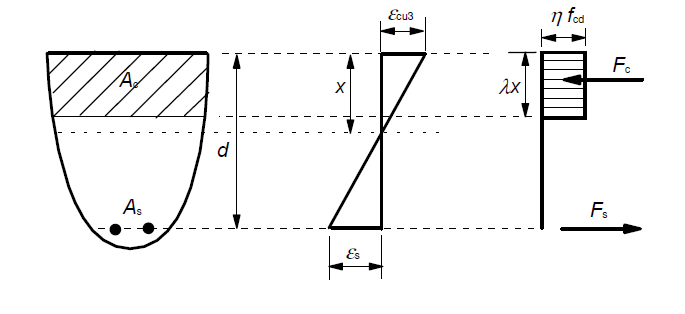
\includegraphics[width=0.9\textwidth]{Figuras/diagrama_tensoes_betao.png} 
    \caption{Diagrama retangular de tensões \cite{EN1992}.}
    \label{fig:diagrama_betao}
\end{figure}

\begin{figure}[htbp]
    \centering
    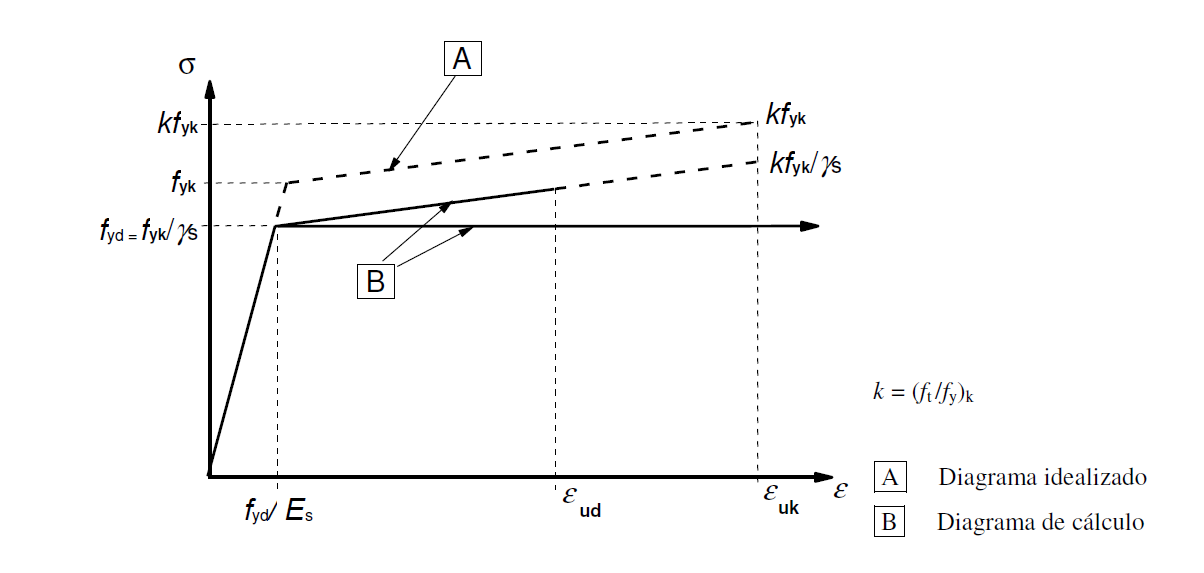
\includegraphics[width=0.9\textwidth]{Figuras/diagrama_aco.png} 
    \caption{Diagramas tensões-extensões, idealizado e de cálculo, do aço das armaduras para betão armado (tracionado ou comprimido) \cite{EN1992}.}
    \label{fig:diagrama_aco}
\end{figure}

\subsubsection{Procedimento de dimensionamento}
Enumeram-se a seguir os passos para efetuar o dimensionamento de elementos em betão armado, nomeadamente, os parâmetros dos materiais, a altura útil da secção, o momento fletor reduzido, a verificação de ductilidade, o cálculo da armadura, e as verificações finais.

\subsubsubsection{Definir as tensões limite para os materiais}
Calcular a tensão de cálculo do betão, através da seguinte expressão,
\begin{equation}
    f_{cd} = \alpha_{cc} f_{ck} / \gamma_{c}
\end{equation}
com  $\alpha_{cc}=1.0$ e $\gamma_{c}=1.5$.\\\\
Calcular a tensão de cedência do aço, com a expressão,
\begin{equation}
    f_{yd} = f_{yk} / \gamma_{s}
\end{equation}
com  $\gamma_{s}=1.15$.\\

\subsubsubsection{Altura útil da secção - $d$}
Assumindo uma estimativa inicial para os diâmetros da armadura, calcular,
\begin{equation}
    d = h - c_{nom} - \phi_{estribo} - \frac{\phi_{long}}{2}
\end{equation}

\subsubsubsection{Momento fletor reduzido - $\mu$}
O momento fletor reduzido caracteriza a solicitação da secção,
\begin{equation}
    \mu = \frac{M_{Ed}}{b \cdot d^{2} \cdot f_{cd}}
\end{equation}

\subsubsubsection{Verificação da ductilidade}
Para evitar armadura de compressão, verificar se $\mu \le \mu_{lim}$. Considerando o limite,
\begin{equation}
    \frac{x}{d} \le 0.45
\end{equation}
para garantir a ductilidade,
\begin{equation}
    \mu_{lim} = 0.8 \cdot 0.45 \cdot (1 - 0.5 \cdot 0.8 \cdot 0.45) \approx 0.295.
\end{equation}
Se $\mu > \mu_{lim}$, a secção deve ser redimensionada.

\subsubsubsection{Cálculo da área total das armaduras - $A_s$}
Calcular a profundidade reduzida do eixo neutro $\xi$ e o braço do binário $z$,
\begin{equation}
    \xi = \frac{1 - \sqrt{1 - 2\mu}}{\lambda},
\end{equation}
\begin{equation}
    z = d \cdot (1 - 0.5 \cdot \lambda \cdot \xi).
\end{equation}
A área de armadura necessária é,
\begin{equation}
    A_s = \frac{M_{Ed}}{z \cdot f_{yd}}
\end{equation}

\subsubsubsection{Verificações finais}
Garantir que,
\begin{equation}
    A_{s} \ge A_{s,min}
\end{equation}
e
\begin{equation}
    A_{s} \le 0.04 A_c
\end{equation}

\subsection{Pilar retangular sujeito a flexão composta reta}
Este modelo destina-se ao dimensionamento de pilares de secção retangular sujeitos a um esforço axial de compressão $N_{Ed}$, e a um momento fletor de cálculo $M_{Ed}$, segundo uma direção principal. O modelo integra a verificação de esbelteza e o cálculo dos efeitos de segunda ordem.

\subsubsection{Dados de Entrada}
\begin{enumerate}
    \item Geometria da secção:\\\\
    $b$ - Largura em \SI{}{mm};\\\\
    $h$ - Altura em \SI{}{mm};\\\\
    $l$ - Comprimento real em \SI{}{mm}.
    \item Condições de apoio:\\\\
    Para definir o coeficiente $\beta$ é necessário definir o tipo de ligação existente no topo e na base do pilar.
    \item Propriedades dos Materiais: \\\\
    $f_{ck}$ - Valor característico da tensão de rotura do betão à compressão aos 28 dias de idade em \SI{}{MPa};\\\\ 
    $f_{yk}$ - Valor característico da tensão de cedência à tração do aço das armaduras para betão armado em \SI{}{MPa};\\\\ 
    $c_{nom}$ - Recobrimento nominal em \SI{}{mm}.
    \item Esforços de cálculo:\\\\
    $N_{Ed}$ - Valor  de cálculo do esforço normal atuante (tração ou compressão) em \SI{}{kN};\\\\
    $M_{Ed}$ - Valor  de cálculo do momento fletor atuante em \SI{}{kNm};\\\\
    $M_{0Ed}$ - Valor do momento fletor de primeira ordem, incluindo o efeito de imperfeições em \SI{}{kNm};\\\\
    $M_{2}$ - Valor do momento nominal de segunda ordem em \SI{}{kNm}.\\
    \item Fluência:\\\\
    Coeficiente de fluência efetivo $\varphi_{ef}$.
\end{enumerate}
Nota: o valor do módulo de elasticidade e/ou de outras constantes são estáticas no algoritmo.

\subsubsection{Procedimento de Cálculo}
Antes do dimensionamento da secção do pilar em betão armado é verificada a sua estabilidade.

\subsubsubsection{Parâmetros de cálculo}
Determinar $f_{cd}$ e $f_{yd}$ e converter os esforços para unidades consistentes (N, mm).

\subsubsubsection{Análise da esbelteza}
\begin{enumerate}
    \item Comprimento de Encurvadura - $l_0$: \\\\
    Determinar por,
    \begin{equation}
        l_0 = \beta \cdot l
    \end{equation}
    onde $\beta$ depende das condições de apoio, e.g.:\\\\
    $\beta=0.7$ para uma apoio encastrado-encastrado;\\\\
    $\beta=2.0$ para uma consola.
    \item Esbelteza - $\lambda$:\\\\
    Calcular o raio de giração,
    \begin{equation}
        i = h / \sqrt{12}
    \end{equation}
    e a esbelteza,
    \begin{equation}
        \lambda = l_0 / i
    \end{equation}
    O valor de $l_0$, para elementos isolados, pode ser determinado utilizando o ábaco apresentado na Figura \ref{fig:esquema_pilar} ou figura 5.7 da EC2-1-1.
    \item Esbelteza limite - $\lambda_{lim}$ \cite{EN1992,CachimBases}:
    \begin{equation}
        \lambda_{lim} = \frac{20 \cdot A \cdot B \cdot C}{\sqrt{n}}
    \end{equation}
    onde,
    \\ $n = N_{Ed} / (A_c f_{cd})$
    \\ $A = 1/(1+0.2\varphi_{ef})$
    \\ $B=1.1$
    \\ $C=0.7$
\end{enumerate}

\begin{figure}[htbp]
    \centering
    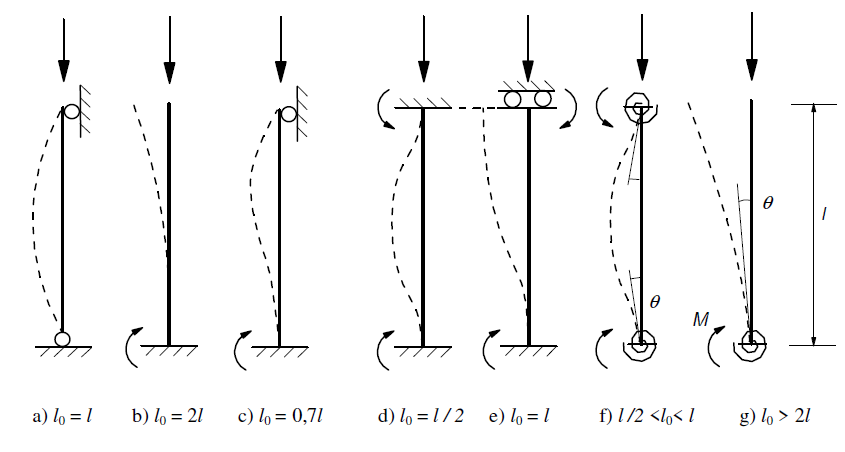
\includegraphics[width=1\textwidth]{Figuras/esquema_pilar_encurvadura.png}
    \caption{Esquema do comprimento de encurvadura para diferentes condições de apoio \cite{EN1992}.}
    \label{fig:esquema_pilar}
\end{figure}

\subsubsubsection{Cálculo do momento fletor - $M_{Ed}$}
Inicialmente $M_{Ed}$ é igual a $M_{0Ed}$.
Se $\lambda > \lambda_{lim}$, i.e., se se tratar de um pilar esbelto, calcular os efeitos de segunda ordem pelo método da curvatura nominal, i.e., calcular,
\begin{enumerate}
    \item a curvatura,
    \begin{equation}
        \frac{1}{r} = K_r \cdot K_{\varphi} \cdot \frac{1}{r_0}
    \end{equation}
    \item a excentricidade de segunda ordem,
    \begin{equation}
        e_2 = \frac{1}{r} \cdot l_0^2 \cdot \frac{1}{c}
    \end{equation}
    \item o momento adicional,
    \begin{equation}
        M_2 = N_{Ed} \cdot e_2
    \end{equation}
    \item e atualizar  o seu valor,
    \begin{equation}
        M_{Ed} = M_{0Ed} + M_2
    \end{equation}
\end{enumerate}

\subsubsubsection{Dimensionamento da armadura}
Com os esforços finais, $N_{Ed}$ e $M_{Ed}$, o método numérico procura, através de um processo iterativo de equilíbrio da secção, uma área de aço para betão $A_s$, tal que:
\begin{itemize}
    \item $N_{Rd} = N_{Ed}$ (equilíbrio axial)
    \item e $M_{Rd} \ge M_{Ed}$ (resistência em flexão composta).
\end{itemize}

\subsubsubsection{Seleção da armadura}
A solução final deve respeitar os limites de armadura mínima e máxima estabelecidos, dados por:
\begin{equation}
    A_{s,min} = \max\left(0.10 \frac{N_{Ed}}{f_{yd}};\, 0.002 A_c\right)
\end{equation}
\begin{equation}
    A_{s,max} = 0.04 A_c
\end{equation}
A área de armadura requerida é assim definida por:
\begin{equation}
    A_{s,req} = \max(A_s;\, A_{s,min})
\end{equation}
com $A_{s,req} \le A_{s,max}$. Por fim, a armadura deve ser disposta de forma simétrica na secção.

\subsection{Sapata isolada e centrada}
Este modelo aplica-se a sapatas de betão armado, de base retangular, suportando um pilar centrado. O procedimento divide-se em duas fases iterativas que a seguir se apresentam - dimensionamento geotécnico (SLS) e dimensionamento estrutural (ELU).

\subsubsection{Dimensionamento geotécnico - SLS}
O objetivo é determinar as dimensões em planta, $a$ e $b$, da sapata de maneira a satisfazer a tensão do solo.

\subsubsubsection{Cálculo dos esforços}
Converter os esforços dos ELU para os dos SLS, dividindo-os por um coeficiente médio, 
\begin{equation}
    \gamma_{G,avg} \approx 1.4
\end{equation}

\subsubsubsection{Ciclo iterativo para a  determinação das dimensões -  $a$ e $b$}
\begin{enumerate}
    \item Inicialmente estimar a área da sapata através do valor de $\sigma_{adm}$.
    \item Em cada iteração, adicionar o peso próprio da sapata às cargas, para determinar a carga total $N_{total}$.
    \item Calcular a excentricidade,
    \begin{equation}
        e = \frac{M_k}{N_{total}}
    \end{equation}
    \item Calcular as tensões no solo,
    \begin{equation}
        \sigma_{max,min} = \frac{N_{total}}{a \cdot b} \cdot \left(1 \pm \frac{6 \cdot e}{b}\right)
    \end{equation}
    \item O ciclo termina quando,
    \begin{equation}
        \sigma_{max} \le \sigma_{adm}
    \end{equation}
    e
    \begin{equation}
        \sigma_{min} \ge 0
    \end{equation}
    sem levantamento, e
    \begin{equation}
        e \le \frac{b}{6}
    \end{equation}
\end{enumerate}

\subsubsection{Dimensionamento estrutural - ELU}
Com a geometria definida na fase anterior, determinar a altura e a armadura da sapata.

\subsubsubsection{Tensão de cálculo}
Calcular
\begin{equation}
    \sigma_{Ed} = \frac{N_{Ed}}{a \cdot b}
\end{equation}
considerando uma distribuição uniforme.

\subsubsubsection{Altura da sapata - Punçoamento}
A altura da sapata é determinada iterativamente para resistir ao punçoamento sem armadura específica:
\begin{enumerate}
    \item Incrementar a altura útil $d$, ver \ref{fig:esquema_puncoamento}.
    \item Calcular o esforço atuante,
    \begin{equation}
        V_{Ed,pun} = N_{Ed} - \sigma_{Ed} \cdot A_{crit}
    \end{equation}
    \item Calcular a resistência $V_{Rd,c}$ do betão.
    \item A altura é válida quando,
    \begin{equation}
        V_{Rd,c} > V_{Ed,pun}
    \end{equation}
\end{enumerate}

\begin{figure}[htbp]
    \centering
    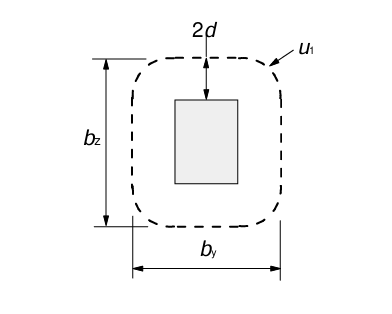
\includegraphics[width=0.6\textwidth]{Figuras/esquema_puncoamento.png}
    \caption{Perímetro de controlo crítico para a verificação ao punçoamento \cite{EN1992}}
    \label{fig:esquema_puncoamento}
\end{figure}

\subsubsubsection{Armaduras de flexão}
A sapata é calculada como consolas nas direções x e y. O momento nas faces do pilar é calculado, e de  seguida é dimensionada a armadura inferior, $A_{s,x}$ e $A_{s,y}$, usando o modelo de flexão simples.

\subsection{Métodos de otimização das armaduras}
Os modelos de otimização das armaduras são aplicados após o dimensionamento de vigas, pilares e sapatas. Os modelos permitem o cálculo da área de aço para betão $A_{s,req}$, através de algoritmos que respeitam as regras de pormenorização da EC2-1-1. Cada um dos modelos corresponde a um tipo de elemento.

\subsection{Otimização de armadura longitudinal (Modelo 1: Vigas e Pilares)}

O Modelo 1 aplica-se a vigas e pilares, baseando-se na otimização por \emph{barras discretas}. O objetivo é encontrar a combinação de varões comerciais (e.g., $4\phi16$) cuja área total $A_{s,\text{prov}}$ seja a mais próxima possível (por excesso) de $A_{s,\text{req}}$, respeitando os espaçamentos mínimos regulamentares.

\subsubsection{Dados de entrada}
\begin{itemize}
\item $A_{s,\text{req}}$: área teórica necessária [\si{cm^2}].
\item $l_d$: largura disponível para armadura:
\begin{equation}
l_d = b - 2(c_\text{nom} + \phi_\text{estribo}).
\end{equation}
\end{itemize}

\subsubsection{Verificação de espaçamento mínimo}
O espaçamento horizontal mínimo é:
\begin{equation}
s_h \geq \max(\phi_\text{long}; 20\,\si{mm}).
\label{eq:sh_min}
\end{equation}

\subsubsection{Geração e seleção de combinações}
O algoritmo gera combinações de varões comerciais por pares:
\begin{itemize}
\item \textbf{Vigas}: de 1 a 4 pares ($\phi$ único ou misto simétrico).
\item \textbf{Pilares}: mínimo 2 pares (garantindo simetria nas 4 faces).
\end{itemize}

De entre as combinações que satisfazem $A_{s,\text{prov}} \geq A_{s,\text{req}}$ e \eqref{eq:sh_min}, seleciona-se a de menor $A_{s,\text{prov}}$.

\subsection{Otimização de armadura distribuída (Modelo 2: Sapatas)}

Nas sapatas, a armadura é calculada por metro linear de largura (e.g., $\phi12@150$\si{mm}). O objetivo é minimizar a taxa de armadura $A_{s,\text{prov}}/m$.

\subsubsection{Dados de entrada}
\begin{itemize}
\item $A_{s,\text{req}}$: área necessária por metro [\si{cm^2/m}].
\item $l$: largura da faixa de cálculo (por defeito, $1\,\si{m}$).
\end{itemize}

\subsubsection{Algoritmo}
\begin{enumerate}
\item Iterar diâmetros comerciais ($\phi10$, $\phi12$, $\phi16$, ...).
\item Para cada $\phi$, calcular $n = \lceil A_{s,\text{req}}/A_\phi \rceil$.
\item Verificar se $n$ varões cabem em $1\,\si{m}$ respeitando espaçamentos.
\item Selecionar combinação com menor $A_{s,\text{prov}}$.
\item Converter em espaçamento: $s = \lfloor 1000/n \rfloor$\si{mm}.
\end{enumerate}
